%! TEX root = ../main.tex
\documentclass[main]{subfiles}

\begin{document}
\chapter{実験4:代理モデル使用時の最適化}
    \section{目的}
    これまでの章で,長野市バス運行スケジュール最適化問題の高速化のために,
    Walsh関数による代理モデルを使用するために必要な要素を決定した.
    本章では,これらの情報を用いて,実際に最適化問題に代理モデルを導入し,高速化が達成できているか検証する.
    ここで,代理モデルを導入した最適化を行った時,どのような結果を得ることが出来れば,高速化が達成できたと言えるのかを確認する.
    図\ref{hv_plot_}は,先行研究でのバス利用率4.5\%の時の世代数ごとのHVを表す.これは図\ref{hv_plot}と同一である.
    
    \begin{figure}
        \centering
        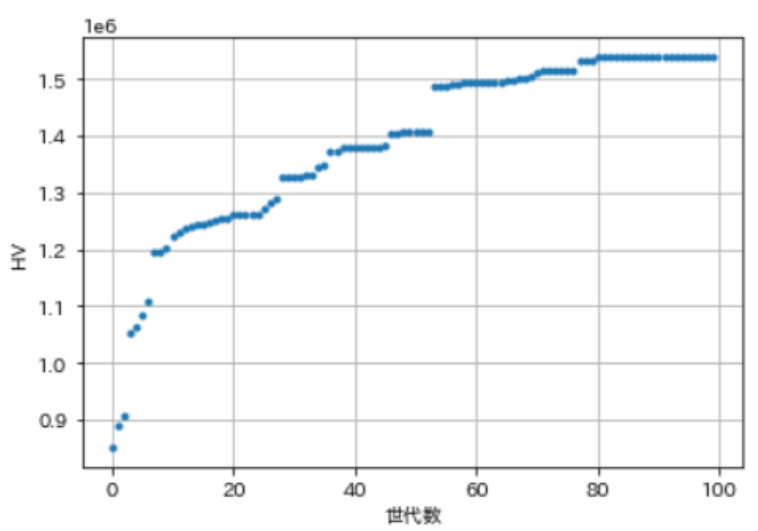
\includegraphics[width=\linewidth]{figures/hv_plot.png}
        \caption{バス利用率4.5\%の場合のHV推移}
        \label{hv_plot_}
    \end{figure}
    先行研究では100世代まで最適化を行い,そのHVが$1.538\times 10^6$であった.
    つまり,代理モデルを導入して最適化を行った結果,
    \begin{itemize}
        \item 100世代目のHVが$1.538\times 10^6$を超える
        \item 100世代目までにHVが$1.538\times 10^6$を超える
    \end{itemize}
    この2つのどちらかを満たしたとき,代理モデルによって最適化を高速化することが出来たと言える.
    
    また,先行研究で使用したアルゴリズムのフローチャートを図\ref{old_algo}に示す.
    \begin{figure}
        \centering
        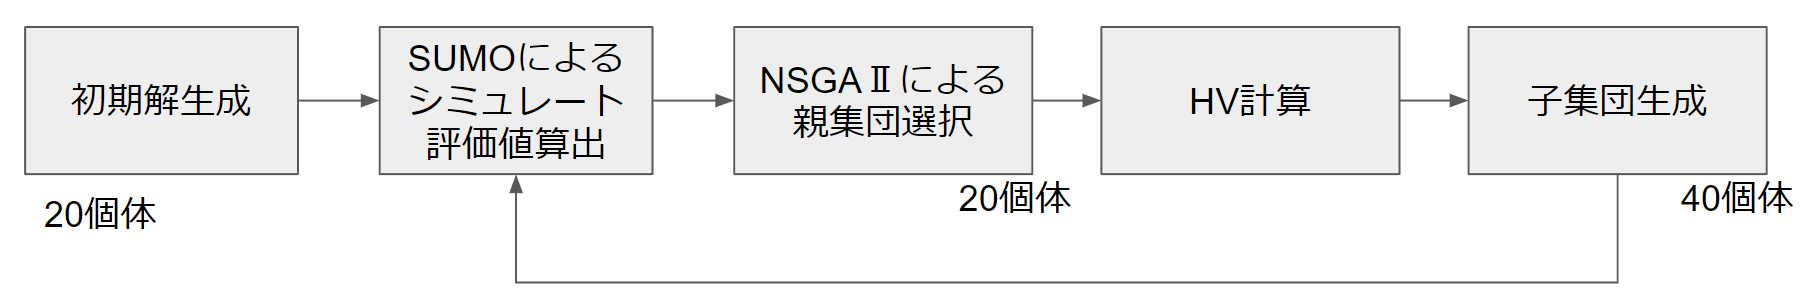
\includegraphics[width=\linewidth]{figures/old_algo.png}
        \caption{先行研究でのアルゴリズムのフローチャート}
        \label{old_algo}
    \end{figure}
    初期解を20個体生成させる.次に,HVを計算し,子集団を20個体生成する.
    新しい解である子集団20個体に対してSUMOによるシミュレートを行い評価値を算出する.
    親集団と子集団合わせた40個体に対し,NSGAⅡにより優れた解20個体を選択する.選ばれた20個体を親集団とする.
    このループを1世代として,ループを100回行うのが先行研究のアルゴリズムである.

    \section{実験方法}
    代理モデルの導入方法について2つの方法を検証した.
    以下でその2つについて,手法のフローチャートと特徴について述べる.
        \subsection{代理モデル内で進化型}
        図\ref{d}にフローチャートを示す.
        \begin{figure}
            \centering
            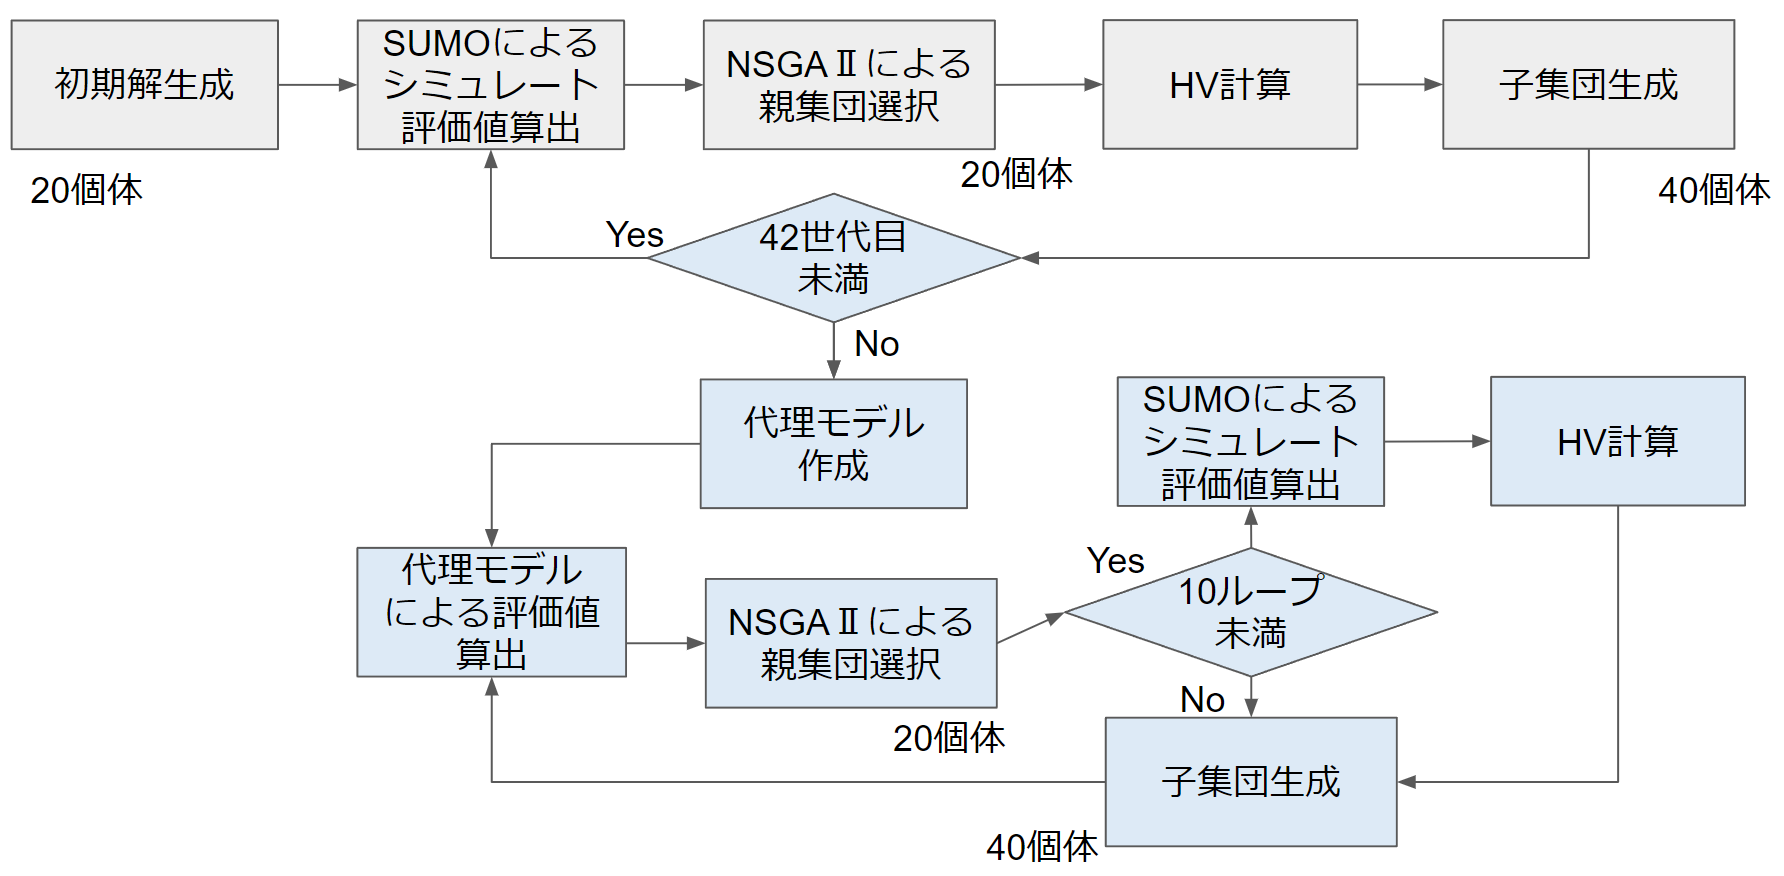
\includegraphics[width=\linewidth]{figures/d.png}
            \caption{代理モデル内で進化型}
            \label{d}
        \end{figure}
        
        図\ref{d}で灰色の要素については図\ref{old_algo}と一致しており,青色の要素が新しく導入された要素である.
        実験3で示したように,41世代目までをWalsh関数の学習データにするため,41世代目までは先行研究と同じアルゴリズムである.
        42世代目で,Walsh関数を用いた代理モデルを作成する.
        そして,代理モデルによって評価値を算出し,親集団を選択,子集団を20個体生成,代理モデルによる評価を繰り返す.
        代理モデルを用いた親集団選択と子集団生成を10ループ行う.
        これは,代理モデルのみを用いて10世代分進化を行っていることと同値である.
        これが,この型の特徴である.
        ただし,最終的なHVの値はSUMOによるシミュレートを用いて評価値を算出し求める.
        代理モデルを用いて10世代分進化を行い,それで得られた個体を,全体の1世代の進化とするのがこの型である.
        ただし,この10世代という値は,なにか定量的な根拠に基づいた数字ではない点について,今後の研究課題であるといえる.
        \subsection{子集団大量生成型}
        図\ref{k}にフローチャートを示す.
        \begin{figure}
            \centering
            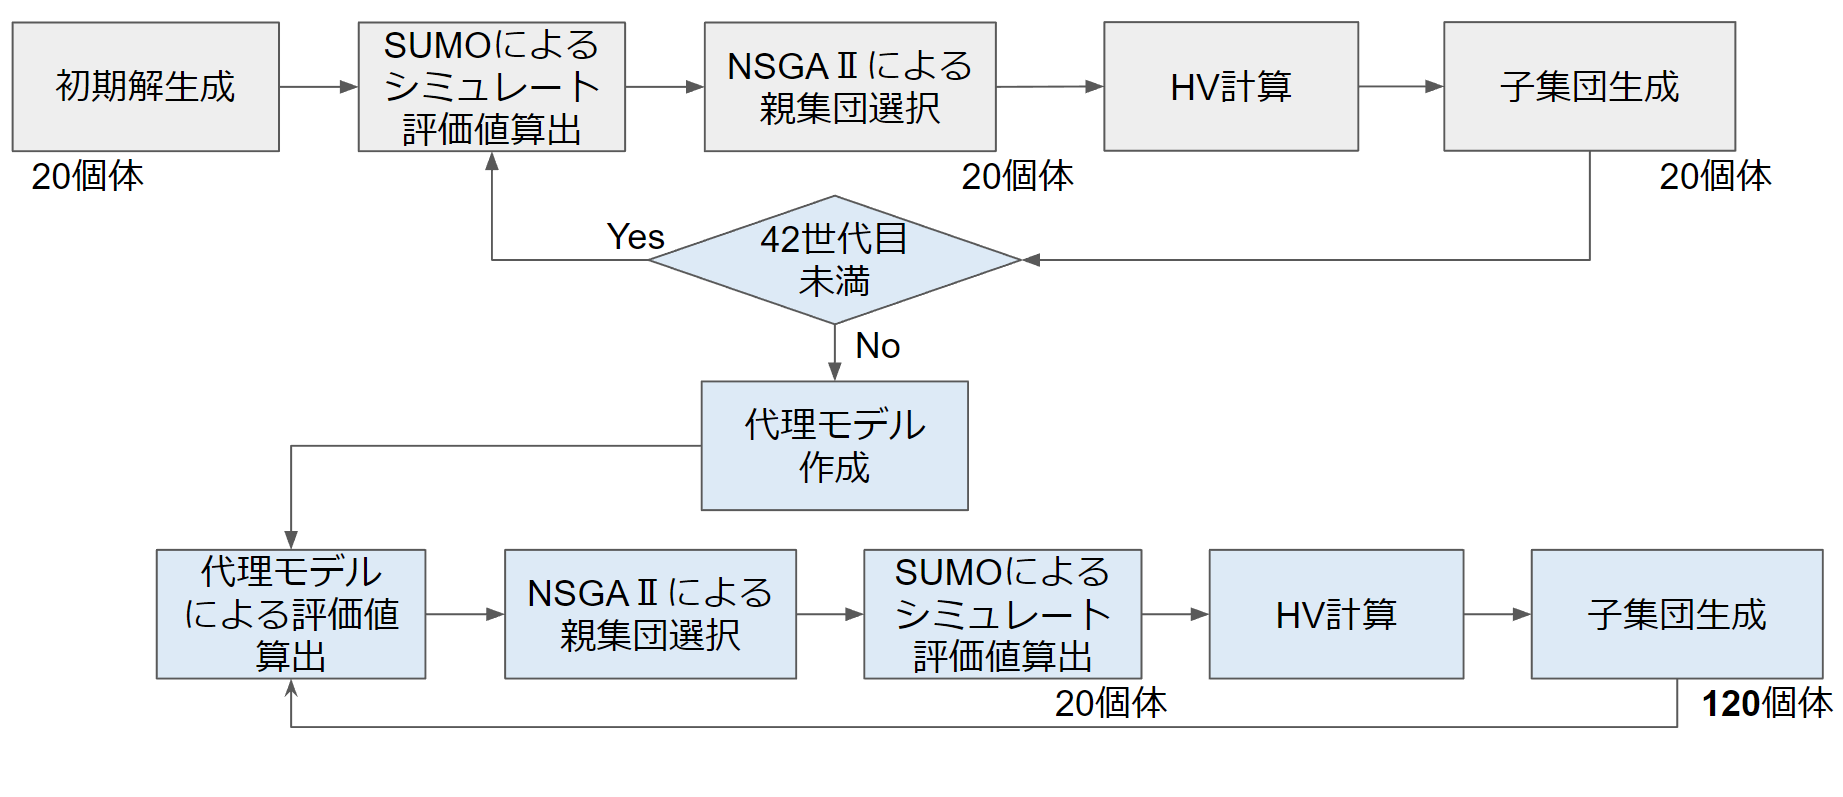
\includegraphics[width=\linewidth]{figures/k.png}
            \caption{子集団大量生成型}
            \label{k}
        \end{figure}

        図\ref{d}で灰色の要素については図\ref{old_algo}と一致しており,青色の要素が新しく導入された要素である.
        青色の要素について,その要素や順番は灰色の要素とほとんど変化がない.
        変化しているところは子集団生成における,生成する子の数である.
        従来では,1世代あたり20個体子を生成していたのに対し,この型では120個体生成している.
        120個体生成しても,代理モデルによって高速に評価できるため,問題なく親集団20個体を選択することが出来る.
        代理モデル内で進化を行うわけでなく,子集団を増やすことで多くの解を生成し,検証するのがこの型の特徴である.
        ただし,代理モデル内で進化型と同じように,120個体という値は,なにか定量的な根拠に基づいた数字ではない点について,今後の研究課題であるといえる.

        両者の型でフローチャートには書かれていないが,1世代ごとに代理モデルは再学習され,代理モデルの精度はより上がっていく.

    \section{結果}
        \subsection{代理モデル内で進化型}
        図\ref{d_result}に結果を示す.
        \begin{figure}
            \centering
            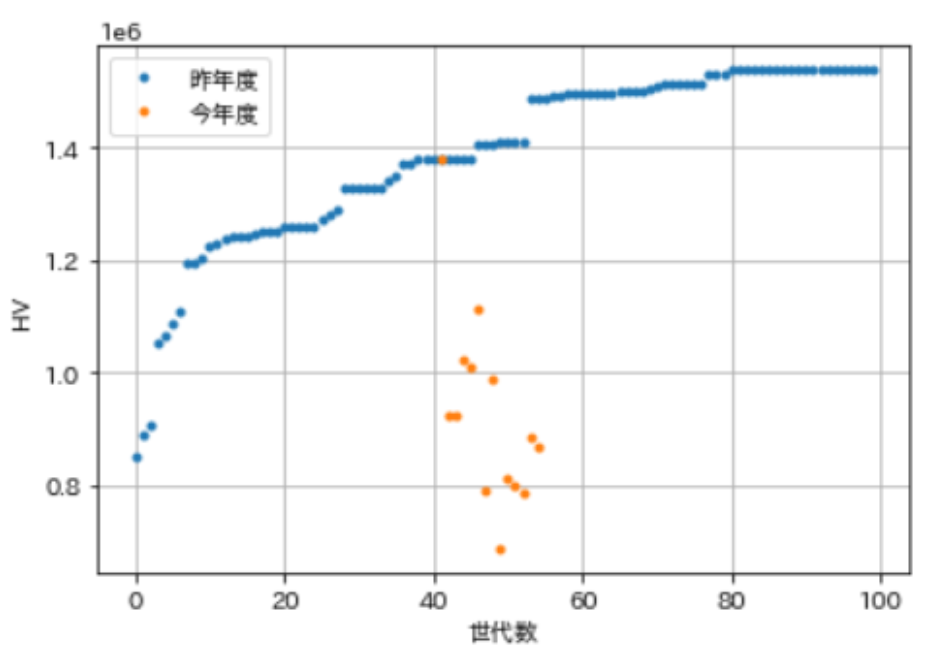
\includegraphics[width=\linewidth]{figures/d_result.png}
            \caption{代理モデル内で進化型の結果}
            \label{d_result}
        \end{figure}

        43世代目以降,今年度のHVが昨年度のHVを上回ることは無かった.
        さらに,HVの値が世代ごとに大きく異なり不安定である.
        \subsection{子集団大量生成型}
        図\ref{k_result}にフローチャートを示す.
        \begin{figure}
            \centering
            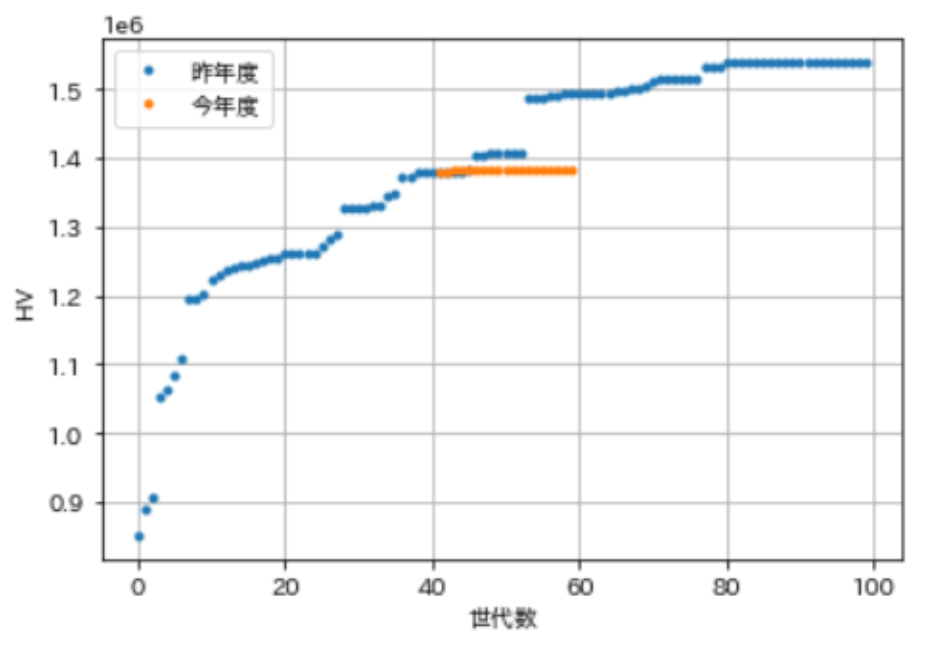
\includegraphics[width=\linewidth]{figures/k_result.png}
            \caption{子集団大量生成型の結果}
            \label{k_result}
        \end{figure}

    \section{考察}
    





\end{document}